\section{Adding New Governing Equations and/or Materials}

There are four basic pieces to adding new physics in the form of a
governing equation or material:
\begin{enumerate}
\item Select the fields for the solution. This will control the form
  of the partial differential equation and the terms in the residuals
  and Jacobians.
\item Derive the point-wise functions for the residuals and
  Jacobians. Determine flags that will be used to indicate which terms
  to include.
\item Determine which parameters in the point-wise functions could
  vary in space as well as any state variables. We bundle all state variables
  and spatially varying parameters into a field called the auxiliary
  field. Each material has a separate auxiliary field.
\item Parameters that are spatially uniform are treated separately
  from the parameters in the auxliary field.
\end{enumerate}

\subsection{Python}

\begin{itemize}
\item Define solution subfields.

  \begin{itemize}
  \item All subfields in the solution field are
    \object{SolutionSubfield} objects (see
    \vref{fig:developer:solution:class}). PyLith already includes
    several solution subfields:
    \begin{description}
    \item[\object{SubfieldDisplacement}] Displacement vector field.
    \item[\object{SubfieldVelocity}] Velocity vector field.
    \item[\object{SubfieldLagrangeFault}] Lagrange multiplier field for
      fault constraints.
    \item[\object{SubfieldPressure}] Fluid pressure or mean stress scalar field.
    \item[\object{SubfieldTemperature}] Temperature scalar field.
    \end{description}
    %
  \item PyLith includes solution field containers with predefined
    subfields:
    \begin{description}
    \item[\object{SolnDisp}] Solution composed of a displacement field.
    \item[\object{SolnDispVel}] Solution composed of displacement and velocity fields.
    \item[\object{SolnDispPres}] Solution composed of displacement and
      mean stress (pressure) fields.
    \item[\object{SolnDispLagrange}] Solution composed of displacement
      and Lagrange multiplier fields.
    \item[\object{SolnDispPresLagrange}] Solution composed of
      displacement, mean stress (pressure), and Lagrange multiplier subfields.
    \item[\object{SolnDispVelLagrange}] Solution composed of
      displacement, velocity, and Lagrange multiplier subfields.
    \end{description}
  \end{itemize}
%
\item Define auxiliary subfields.

  The auxiliary subfields for a material are defined as facilities in
  a Pyre Component. For example, the ones for
  \object{IsotropicLinearElasticityPlaneStrain} are in
  \object{AuxFieldIsotropicLinearElasticity}. The order of the subfields
  is defined {\em not} by the order they are listed in the Pyre
  component, but by the order they are added to the auxiliary field in
  the C++ object.

\item Flags to turn on/off terms in governing equation.

  For the elasticity equation, we sometimes do not include body forces
  or inertial terms in our simulations. Rather than implement these
  cases as separate materials, we simply include flags in the material
  to turn these terms on/off. The flags are implemented as Pyre
  properties in our material component.
\end{itemize}

\begin{figure}[htbp]
  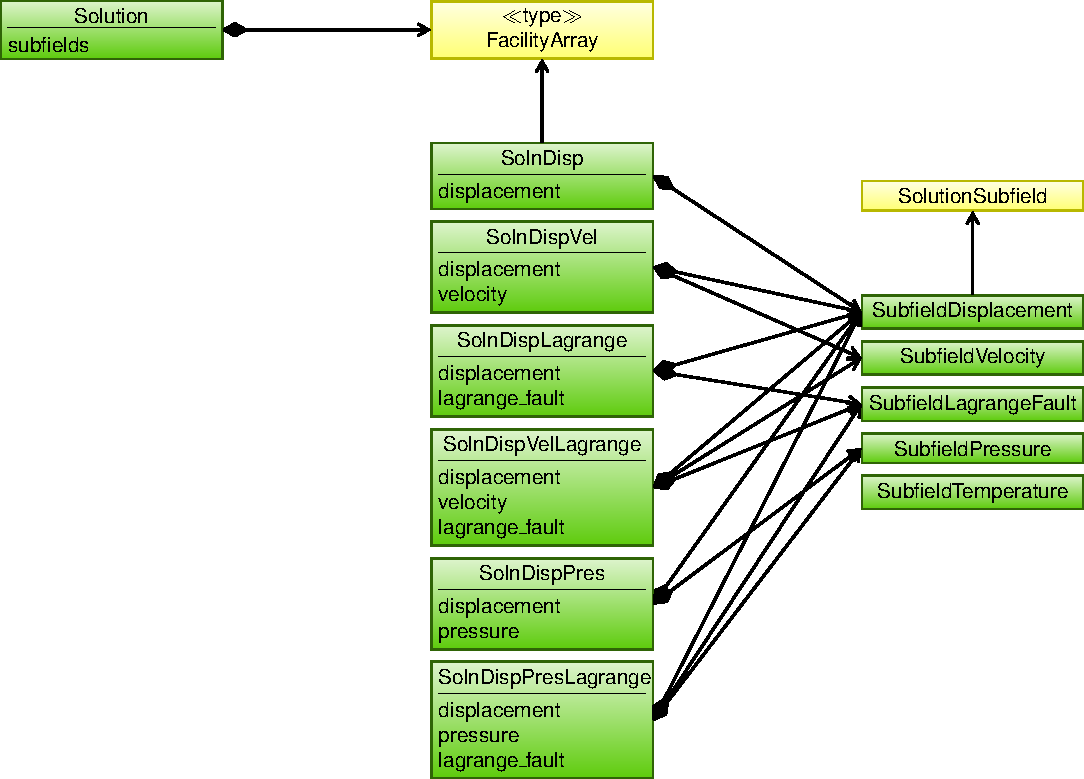
\includegraphics[scale=0.8]{developer/figs/solution_classdiagram}
  \caption{Class diagram for the solution field, solution subfields,
    and pre-defined containers of solution subfields.}
  \label{fig:developer:solution:class}
\end{figure}

\subsection{C++}

\warning{We will likely be refactoring the \object{Material} and
  \object{IntegratorPointwise}, so how the point-wise functions for
  the residual, Jacobians, state variable update, and computation of
  derived fields are set will likely be significantly different and
  easier in the future. For now, you should use
  \object{IsotropicLinearElasticityPlaneStrain} as a model for how to
  implement a material.}

\begin{itemize}
\item Define auxiliary subfields.

  We build the auxiliary field using classes derived from
  \object{pylith::feassemble::AuxiliaryFactory}. The method
  corresponding to each subfield specifies the name of the subfield,
  its components, and scale for nondimensionalizing. We generally
  create a single auxiliary factory object for each governing equation
  but not each bulk constitutive model, because constitutive models
  for the same governing equation often have many of the same
  subfields. For example, most of our bulk constitutive models for the
  elasticity contain density, bulk modulus, and shear modulus
  auxiliary subfields.

  \important{Within the concrete implementation of the material
    object, we add the subfields to the auxiliary field. The order in
    which they are added determines the order they will be in the
    auxiliary field. You will need to use know this order when you
    implement the point-wise functions.}

\item Implement the point-wise functions.

  The point-wise functions for the residuals, Jacobians, and
  projections follow nearly identical interfaces. Note that within
  PyLith, we use PylithInt, PylithReal, and PylithScalar instead of
  PetscInt, PetscReal, and PetscScalar.

\item Set the point-wise functions.

  We set the point-wise functions for the residual using
  \object{PetscDSSetResidual} and for the Jacobian using
  \object{PetscDSSetJacobian}.

\end{itemize}

\begin{figure}[htbp]
  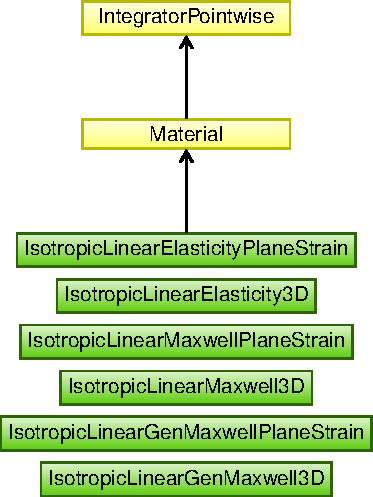
\includegraphics[scale=0.8]{developer/figs/material_classdiagram}
  \caption{Class diagram for the bulk materials. Each material
    implementation inherits from the abstract \object{Material} class
    which inherits from the abstract \object{IntegratorPointwise}
    class.}
  \label{fig:developer:material:class}
\end{figure}

\subsection{C++ Unit Tests}

The C++ unit tests focus on testing all methods of a C++ object. In
most cases, this includes the accessors, layout and values of the
auxiliary field, the residual, and Jacobian. For the residual and
Jacobian, we use the method of manufactured solutions. In testing the
residual, we manufacture a solution that solves the governing
equation. We setup the object so that the auxiliary field and solution
passed to the residual computation should produce a zero residual
vector. The \object{UserFunctionDB} spatial database allows us to
populate the auxiliary field and solution using anlytical
functions. To test the computation of the RHS Jacobian, we compute
\begin{equation}
    J_g(s) (p - s) = G(p) - G(s),
\end{equation}
where $J_g(s)$ is the RHS Jacobian, $s$ is a solution to the governing
equation, $p$ is $s$ plus a small perturbation, $G(p)$ is the RHS
residual for $p$, and $G(s)$ is the RHS residual for $s$. We test the
computation of the LHS Jacobian, using the corresponding LHS Jacobian
$J_f$ and LHS residual $F$.

\important{In setting up a test using the Method of Manufactured Solutions it is important to make sure the
discretization of the used for each of the subfields in the auxiliary field and solution field are sufficient to
represent the analytical function.}


\begin{figure}[htbp]
  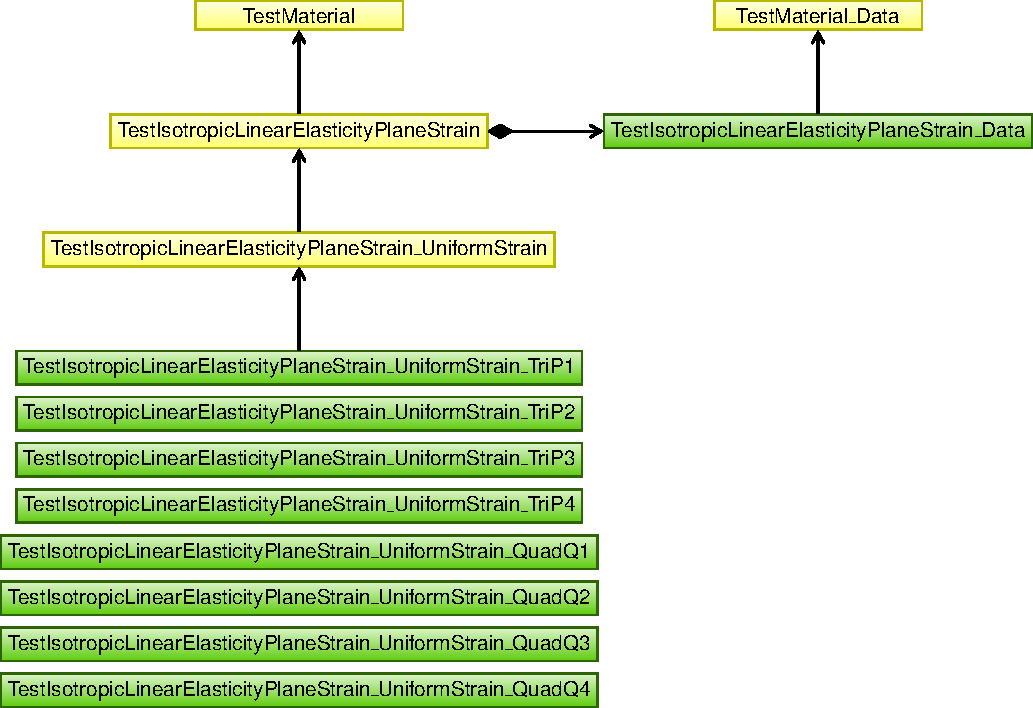
\includegraphics[scale=0.8]{developer/figs/testmaterial_classdiagram}
  \caption{Class diagram for testing the
    \object{IsotropicLinearElasticityPlaneStrain} material with a
    solution generated using the Method of Manufactured
    Solutions. \object{TestIsotropicLinearElasticityPlaneStrain\_UniformStrain}
    contains the parameters and generated solution and the subclasses
    include various discretizations. All of the test data is held in
    the \object{TestIsotropicLinearElasticityPlaneStrain\_Data}
    object.}
  \label{fig:developer:test:material:class}
\end{figure}


\subsection{Python Unit Tests}

With the Python implementation focused on gathering the user configuration of a simulation, there is
minimal functionality we can test at the Python level. Consequently, the Python unit tests are generally
limited to testing the SWIG interface, which involves creating the C++ object and insuring the Pyre
properties and facilities and any other information is passed to the C++ object.


% End of file
